\chapter{Comparison theorems for \pch}


\section{Finite type algebras}
\label{sec:1.1}

We will compare the \pch of certain finite type algebras and completions thereof. 
The motivating example of the result we aim at is as follows.

Let $X$ be a nonsingular complex affine variety. We consider the
algebras $\mc O (X)$ of regular (polynomial) functions and
$C^\infty (X)$ of complex valued smooth functions on $X$. By
default, if we talk about continuous or differentiable functions on
$X$ or about the cohomology of $X$, we always do this with respect
to the analytic topology on $X$, obtained from embedding $X$ in a
complex affine space.

The Hochschild--Kostant--Rosenberg--Connes theorem tells us what the
\pch of these algebras looks like:
\begin{equation}\label{eq:1.1}
\begin{array}{lll}
HP_n (\mc O (X)) & \cong &
\bigoplus_{m \in \mh Z} H_{DR}^{n+2m} (X ; \mh C) \,, \\
HP_n (C^\infty (X)) & \cong &
\bigoplus_{m \in \mh Z} H_{DR}^{n+2m} (X ; \mh C) \,.
\end{array}
\end{equation}
In the first line we must take the De Rham cohomology of $X$ as an
algebraic variety. However, according to a result of Grothendieck
and Deligne this is naturally isomorphic to the De Rham cohomology
of $X$ as a smooth manifold. Hence the inclusion $\mc O (X) \to
C^\infty (X)$ induces an isomorphism
\begin{equation}
HP_* (\mc O (X)) \to HP_* (C^\infty (X)) \,.
\end{equation}
Now let us discuss this in greater generality, allowing
noncommutative algebras. We denote the primitive ideal spectrum of
any algebra $A$ by Prim$(A)$ and we endow it with the Jacobson
topology, which is the natural noncommutative generalization of the
Zariski topology. An algebra homomorphism $\phi : A \to B$ is called
spectrum preserving if it induces a bijection on primitive ideal spaces,
in the following sense. For every $J \in \mr{Prim}(B)$ there is a 
unique $I \in \mr{Prim}(A)$ such that $\phi^{-1}(J) \subset I$,
and the map Prim$(B) \to \mr{Prim}(A) : J \mapsto I$ is bijective.

Since we do not want to get too far away from commutative
algebras, we will work with finite type algebras, see
\cite{KNS,BaNi}. Let $\mb k$ be the ring of regular functions on
some complex affine variety. A finite type $\mb k$-algebra is a
$\mb k$-algebra that is finitely generated as a $\mb k$-module.
The \pch of a finite type algebra always has finite dimension,
essentially because this is case for $\mc O (X)$ \cite[Theorem 1]{KNS}. 
Moreover it depends only on the primitive ideal spectrum
of the algebra, in the following sense:

\begin{thm}\label{thm:1.1} \textup{\cite[Theorem 8]{BaNi}}\\
A spectrum preserving morphism of finite type $\mb k$-algebras
induces an isomorphism on \pch \!.
\end{thm}

Morally speaking $HP_* (A)$ should correspond to the ``cohomology'' of Prim$ (A)$.
However, this is only a nonseparated scheme, so classical cohomology theories will 
not do. Yet this can be made precise with sheaf cohomology \cite[Section 2.2]{Sol3}.

It is not unreasonable to expect that there is always some
Fr\'echet completion $A\sm$ of $A = A\al$ such that the inclusion 
$A\al \to A\sm$ induces an isomorphism
\begin{equation}\label{eq:1.4}
HP_* (A\al ) \to HP_* (A\sm ) \,.
\end{equation}
A good candidate appears to be
\begin{equation}
A\sm = A\al \otimes_{\mc O (X)} C^\infty (X)
\end{equation}
if the center of $A\al$ is $\mc O (X)$. However I believe that it
would be rather cumbersome to determine precisely under which conditions this
works out. Moreover I do not know whether the resulting smooth
algebras are interesting in this generality. Therefore we restrict
our attention to algebras of a specific (but still rather general) form,
which we will now describe.

Let $\Gamma$ be a finite group acting (by $\alpha$) on the nonsingular
complex affine variety $X$. Take $N \in \mh N$ and consider the
algebra of matrix-valued regular functions on $X$:
\begin{equation}
\mc O (X ; M_N (\mh C) ) := M_N (\mc O (X)) =
\mc O (X) \otimes M_N (\mh C ) \,.
\end{equation}
Suppose that we have elements $u_\gamma \in GL_N (\mc O (X))$ such that
\begin{equation}\label{eq:1.2}
(\gamma \cdot f) (x) = u_\gamma (x) f (\alpha_\gamma^{-1} x)
u_\gamma^{-1} (x)
\end{equation}
defines a group action of $\Gamma$ on $M_N (\mc O (X))$, by
algebra homomorphisms. We do not require that $\gamma \mapsto
u_\gamma$ is a group homomorphism. Nevertheless the above does imply 
that there exists a 2-cocycle $\lambda : \Gamma \times \Gamma \to \mc O
(X)^\times$ such that
\[
u_\gamma (u_{\gamma'} \circ \alpha_\gamma^{-1}) =
\lambda (\gamma , \gamma') u_{\gamma \gamma'} \,.
\]
In particular, for every $x \in X$ we get a projective $\Gamma_x$-representation
\begin{equation}\label{eq:1.18}
(\pi_x ,\mh C^N ) \quad \mr{with} \quad \pi_x (\gamma ) = u_\gamma (x) \,.
\end{equation}
The element $u_\gamma$ should be regarded as an intertwiner
between representations with $\mc O (X)$-characters $x$ and
$\alpha_\gamma (x)$. We are interested in the finite type algebra
\begin{equation}\label{eq:1.13}
A\al = \mc O (X ; M_N (\mh C ))^\Gamma
\end{equation}
of $\Gamma$-invariant elements. We note that restriction of a
module from $A\al$ to $\mc O (X)^\Gamma$ defines a continuous
finite to one surjection \cite[Lemma 1]{KNS}
\begin{equation}\label{eq:1.3}
\theta : \mr{Prim}(A\al ) \to X / \Gamma \,.
\end{equation}
\textbf{Examples.}\\
Classical algebras of this type are
\begin{equation}\label{eq:1.14}
\begin{array}{lll}
\mc O (X)^\Gamma & = & \mc O (X / \Gamma ) \,, \\
\mc O \big( X ; \mr{End} (\mh C [\Gamma]) \big)^\Gamma
& \cong & \mc O (X) \rtimes \Gamma \,.
\end{array}
\end{equation}
For example, take $X = \mh C^3$ and $\Gamma = \mh Z / 3 \mh Z$,
acting through cyclic permutations of the coordinates. Put $A\al =
\mc O (X) \rtimes \Gamma$.  Almost all points $\Gamma x \in X /
\Gamma$ correspond to a unique irreducible $A\al$-module,
namely $\mr{Ind}_{\mc O (X)}^{A\al} \mh C_x$. Only the points
$(z,z,z)$ with $z \in \mh C$ carry three irreducible $\mc O (X)
\rtimes \Gamma$-modules, of the form $\mh C_{(z,z,z)} \otimes \mh
C_{\zeta}$ with $\zeta$ a cubic root of unity.
\\[2mm]
More generally, suppose that we have a larger group $G$ with a
normal subgroup $N$ such that $\Gamma = G / N$. Let $(\pi ,V)$ be a
$G$-representation on which $N$ acts by a character. Then
\[
(g \cdot f)(x) = \pi (g) f (\alpha_{g N}^{-1} x) \pi (g^{-1})
\]
defines an action of $G$ on $\mc O (X ; \mr{End} (V))$ which
factors through $\Gamma$, so
\[
\mc O (X ; \mr{End} (V))^G = \mc O (X ; \mr{End} (V))^\Gamma \,.
\]
If we put $u_\gamma = \pi (g)$ for some $g$ with $g N = \gamma$
then we are in the setting of \eqref{eq:1.2}. Yet in general
there is no canonical choice for $u_\gamma$, and we end up with a
nontrivial cocycle $\lambda$. (In fact this a typical example of a
projective $\Gamma$-representation.)\\[2mm]

The natural Fr\'echet completion of \eqref{eq:1.13} is
\begin{equation}\label{eq:1.22}
A\sm = C^\infty (X ; M_N (\mh C))^\Gamma \,.
\end{equation}
This algebra has the same spectrum as $A\al$, but the two algebras 
induce different Jacobson topologies on this set. The Jacobson 
topology from $A\sm$ is finer, and makes Prim$ (A\sm )$ a non-Hausdorff manifold. 
(By this we mean a second countable topological space in which every point has a
neighborhood that is homeomorphic to $\mh R^n$.)

The map \eqref{eq:1.4} is an isomorphism in the special cases where 
$A\al$ is as in \eqref{eq:1.14} and $A\sm$
as in \eqref{eq:1.22}, as follows from comparing \cite{KNS} and
\cite{Was}. We will show that it holds much more generally, for
example if we take $A\sm = C^\infty (X' ; M_N (\mh C))^\Gamma$
with $X'$ a suitable deformation retract of $X$. Such an algebra
is finitely generated as a $C^\infty (X')^\Gamma$-module, and
therefore we will call it a (topological) finite type algebra.
\vspace{4mm}





\section{The commutative case}
\label{sec:1.2}

Let $CC_{**}(A)$ be the periodic cyclic bicomplex associated to an algebra $A$
\cite[Section 1]{Lod}. Its terms are of the form $A^{\otimes n}$ and its homology
is by definition $HP_* (A)$.
For topological algebras we must specify which particular topological
tensor product we wish to use in cyclic theory. By default we work with a
Fr\'echet algebra $A$ whose topology is defined by
submultiplicative seminorms, and with the completed projective
tensor product $\hot$. Since this is a completion of the algebraic
tensor product we get natural maps
\[
\begin{array}{lll}
CC_{**}(A , \otimes) & \to & CC_{**}(A ,\hot) \,, \\
HP_* (A , \otimes) &\to & HP_* (A ,\hot) \,.
\end{array}
\]
We abbreviate $CC_{**}(A) = CC_{**}(A ,\hot)$ and $HP_* (A) = HP_* (A ,\hot )$ for Fr\'echet
algebras. Recall that an extension of topological algebras is admissible if it is split 
exact in the category of topological vector spaces. An ideal $I$ of $A$ is admissible if\\ 
$0 \to I \to A \to A/I \to 0$ is admissible. 

Any extension $0 \to A \to B \to C \to 0$ gives rise to a short exact sequence of
differential complexes
\begin{align*}
& 0 \to CC_{**}(B,A) \to CC_{**}(B) \to CC_{**}(C) \to 0 \,, \\
& CC_{**}(B,A) := \ker \big( CC_{**}(B) \to CC_{**}(C) \big) \,.
\end{align*}
By a standard construction in homological algebra this leads to a long exact sequence
\begin{equation}\label{eq:1.19}
\cdots \to HP_i (B,A) \to HP_i (B) \to HP_i (C) \to HP_{i+1}(B,A) \to \cdots
\end{equation}
Actually this sequence wraps up to an exact hexagon, because $HP_{i+2} \cong HP_i$.
The inclusion $CC_{**}(A) \to CC_{**}(B,A)$ induces a map $HP_* (A) \to HP_* (B,A)$.
One of our main tools will be the excision property of \pch \!:

\begin{thm}\label{thm:1.2}
Let $0 \to A \to B \to C \to 0$ be an extension of \textup{(}nontopological\textup{)}
algebras or an admissible extensions of Fr\'echet algebras. Then $HP_* (A) \to HP_* (B,A)$
is an isomorphism, and \eqref{eq:1.19} yields an exact hexagon
\[
\hexagon{HP_0 (A)}{HP_0 (B)}{HP_0 (C)}{HP_1 (C)}{HP_1 (B)}{HP_1 (A)}
\]
\end{thm}
\emph{Proof.}
The basic version of this theorem is due to Wodzicki \cite{Wod}.
It was proved in general by Cuntz and Quillen \cite{CuQu,Cun}.
$\qquad \Box$ \\[2mm]

Suppose that we want to prove that an algebra homomorphism
$\phi : A \to B$ induces an isomorphism on $HP_*$. The excision
property can be used as follows:

\begin{lem}\label{lem:1.3}
Suppose that there are sequences of ideals
\begin{align*}
& A = \, I_0 \supset \, I_1 \supset \cdots \supset I_d = 0 \\
& B = J_0 \supset J_1 \supset \cdots \supset J_d = 0
\end{align*}
with the properties
\begin{itemize}
\item $\phi (I_p ) \subset J_p$ for all $p \geq 0$,
\item $HP_* (I_{p-1} / I_p ) \to HP_* (J_{p-1} / J_p)$ is an
isomorphism for all $p \geq 0$,
\item if $B$ \textup{(}respectively $A$\textup{)} is Fr\'echet then the ideals
$J_p$ \textup{(}respectively $I_p$\textup{)} are admissible.
\end{itemize}
Then $HP_* (\phi) : HP_* (A) \to HP_* (B)$ is an isomorphism.
\end{lem}
\emph{Proof.}
Left as an exercise. Use the five lemma. $\qquad \Box$
\\[2mm]

Generally speaking a good tool to compute the \pch of a
finite type algebra $A$ is a filtration by ideals $I_p$ such that
the successive quotients $I_{p-1} / I_p$ behave like
commutative algebras. In particular Prim$ (I_{p-1}/I_p )$
should be a (separated) affine variety, so this gives rise a
kind of stratification of Prim$ (A)$. This can be formalized with the notion of 
an abelian filtration \cite{KNS}.

To describe suitable smooth analogues of $A\al$ we must say what
precisely we mean by smooth functions on spaces that are not
manifolds. Let $Z \subset Y$ be subsets of a smooth manifold $X$ and let
$V$ be a complete topological vector space.
\[
\begin{array}{lll}
C^\infty (Y ; V) & := & \big\{ f : Y \to V \,|\, \exists \text{
open } U \subset X , \tilde f \in C^\infty (U ; V) :
Y \subset U , \tilde f \big|_Y = f \big\} \\
C^\infty_0 (Y,Z) & := &
\{ f \in C^\infty (Y ; \mh C) : f \big|_Z = 0 \} \\
C^\infty_0 (Y,Z;V) & := & \{ f \in C^\infty (Y ; V) : f \big|_Z = 0 \}
\end{array}
\]
Recall that a corner in a manifold is a point that has a neighborhood 
homeomorphic to $\mh R^n \times [0,\infty )^m$, with $m > 0$. To 
apply excision we will often need the following result of Tougeron:

\begin{thm}\label{thm:1.9} \textup{\cite[Th\'eor\`eme IX.4.3]{Tou}}\\
Let $Y$ be a smooth manifold and $Z$ a smooth submanifold, both
possibly with corners. The following extension is admissible:
\[
0 \to C_0^\infty (Y,Z) \to C^\infty (Y) \to C^\infty (Z) \to 0 \,.
\]
\end{thm}

For completeness we include an extended version of the Hochschild--Kostant--Rosenberg
theorem for \pch \!. We abbreviate
\[
H^{[n]}(Y) = {\ts \bigoplus_{m \in \mh Z}} \check H^{n+2m}(Y ; \mh C) \,.
\]
\begin{thm}\label{thm:1.8}
Let $Y$ be a smooth manifold, possibly noncompact and with corners.
There is a natural isomorphism 
\[
HP_* (C^\infty (Y)) \cong H^{[*]}(Y ) \,.
\]
\end{thm}
\emph{Proof.} 
For $Y$ compact and without boundary this is due to Connes \cite[p. 130]{Con}, who in fact
proved the much stronger statement
\begin{equation}\label{eq:1.15}
HH_* (C^\infty (Y)) \cong \Omega^* (Y) \,.
\end{equation}
Here $HH_*$ denotes Hochschild homology and $\Omega^*$ means differential forms with 
complex values. By Corollary 4.3 and Theorem 7.1 of \cite{BLT} \eqref{eq:1.15} still holds if
$Y$ is allowed to have corners and may be noncompact. Hence $HP_* (C^\infty (?))$ and 
$H^{[*]} (? )$ agree at least locally. By Theorems \ref{thm:1.2} and \ref{thm:1.9} both
these functors satisfy excision, so they agree on every manifold. $\qquad \Box$
\\[2mm]

Let $Y$ be a complex affine variety and $Z$ a closed subvariety,
both possibly reducible and singular. In line with the above we write
\[
\begin{array}{lll}
\mc O_0 (Y,Z) & := & \{ f \in \mc O (Y) : f \big|_Z = 0 \} \,, \\
\mc O_0 (Y,Z;V) & := & O_0 (Y,Z) \otimes V \,.
\end{array}
\]
Let $\check H^* (Y,Z;\mh C )$ denote the \v Cech cohomology of the pair
$(Y,Z)$, with complex coefficients and with respect to the analytic
topology. Because $HP_*$ and $K_*$ have a $\mh Z / 2 \mh Z$-grading,
it is convenient to impose this also on \v Cech cohomology. Therefore we write
\begin{equation}\label{eq:1.6}
H^{[n]} (Y,Z) := {\ts \bigoplus_{m \in \mh Z}} \check H^{n+2m} (Y,Z;\mh C )
\end{equation}
Now we are ready to state and prove the comparison theorem
for the \pch of commutative algebras.

\begin{thm}\label{thm:1.4}
\begin{description}
\item[a)] There is a natural isomorphism
$HP_* \big( \mc O_0 (Y,Z) \big) \cong H^{[*]} (Y,Z)$.
\item[b)] Suppose that $Y \setminus Z$ is nonsingular and that
$\tilde C_0^\infty (Y,Z)$ is a Fr\'echet algebra with the properties
\item[$\bullet$] $\mc O_0 (Y,Z) \subset \tilde C_0^\infty (Y,Z) \subset
C_0^\infty (Y,Z)$ \,,
\item[$\bullet$] if the partial derivatives of $f \in C_0^\infty (Y,Z)$ all
vanish on $Z$ then $f \in \tilde C_0^\infty (Y,Z)$.\\
Then $HP_* (\mc O_0 (Y,Z)) \to HP_* \big( \tilde C_0^\infty (Y,Z) \big)$ 
is an isomorphism.
\end{description}
\end{thm}
\emph{Proof.}
a) was proved in \cite[Theorem 9]{KNS}.\\
b) By assumption $Y\setminus Z$ with the analytic topology is a smooth manifold. 
Let $N$ be a closed neighborhood of $Z$ in $Y$, such that $Y \setminus N$ is a 
smooth manifold and a deformation retract of $Y \setminus Z$. Let 
$r : [0,1] \times Y \to Y$ be a smooth map with the properties
\begin{enumerate}
\item $r_1 = \mr{id}_Y$ where $r_t (y) := r(t,y) $,
\item $r_t (z) = z \; \forall z \in Z , t \in [0,1] $,
\item $r_t (N) \subset N \; \forall t \in [0,1]$ and $r_0 (N) = Z $,
\item $r_t^{-1} (Z)$ is a neighborhood of $Z \; \forall t < 1 $,
\item $r_t \colon r_t^{-1}(Y \setminus Z) \to Y \setminus Z$ is a
diffeomorphism $\forall t \in [0,1] $.
\end{enumerate}
Consider the algebra homomorphisms
\[
\begin{array}{lll@{\qquad}lll}
C_0^\infty (Y,N) & \to & \tilde C_0^\infty (Y,Z), & f & \to & f \,, \\
\tilde C_0^\infty (Y,Z) & \to & C_0^\infty (Y,N), &
f & \to & f \circ r_0 \,.
\end{array}
\]
By construction these are diffeotopy equivalences. The diffeotopy
invariance of $HP_* (?,\hot )$ \cite[p. 125]{Con} ensures that
\[
HP_* \big( \tilde C_0^\infty (Y,Z) \big) \cong
HP_* \big( C_0^\infty (Y,N) \big) \,.
\]
Write $\tilde Y = r_{1/2}^{-1} (Y \setminus Z)$ and
$\tilde N = N \cap \tilde Y$. This could look like
\\[1mm]
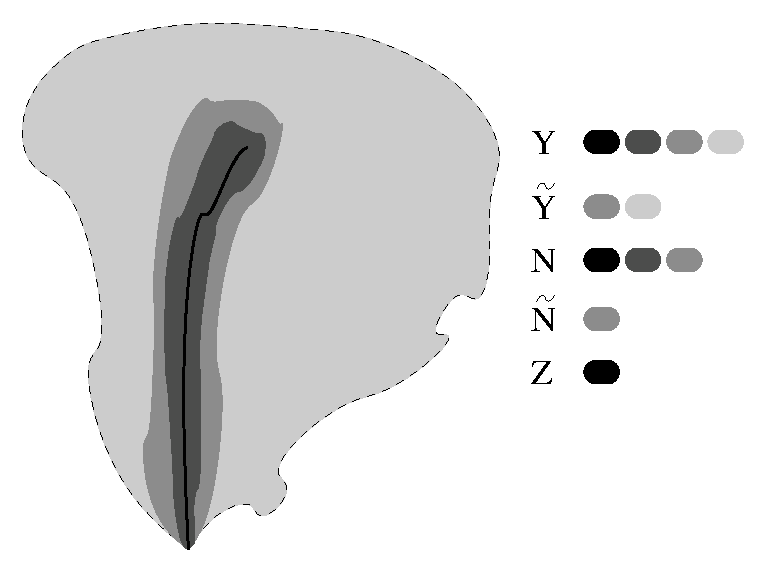
\includegraphics[width=8cm,height=5cm]{ynz}

\noindent By Theorem \ref{thm:1.9} there is an admissible extension
\[
0 \to C_0^\infty (Y,N) = C_0^\infty \big( \tilde Y , \tilde N \big)
\to C^\infty \big( \tilde Y \big) \to C^\infty \big( \tilde N \big)
\to 0 \,.
\]
Combining this with Theorems \ref{thm:1.2} and \ref{thm:1.8} yields natural
isomorphisms
\[
HP_* \big( C^\infty (\tilde Y ,\tilde N) \big) \cong H^{[*]} \big(
\tilde Y ,\tilde N \big) \cong H^{[*]} (Y,N) \cong H^{[*]} (Y,Z) \,.
\]
Now consider the diagram
\[
\begin{array}{ccc}
HP_* (\mc O_0 (Y,Z)) & \cong & H^{[*]} (Y,Z) \\
\downarrow & & || \\
HP_* \big( C^\infty (\tilde Y ,\tilde N) \big) & \cong &
H^{[*]} (Y,Z)
\end{array}
\]
It commutes by naturality, so the arrow is an isomorphism.
$\qquad \Box$
\vspace{4mm}




\section{Comparison with topological $K$-theory}
\label{sec:1.3}

Let $\Gamma$ be a finite group which acts by diffeomorphisms on a 
smooth manifold $X$. We will frequently meet algebras of the form
\begin{equation}\label{eq:1.5}
C_0^\infty (Y,Z;M_N (\mh C) )^\Gamma
\end{equation}
where $Y$ and $Z$ are $\Gamma$-stable closed submanifolds of $X$.
We allow our manifolds to have corners (and in particular a
boundary), since these appear naturally in orbifolds. But we must
be careful, because the algebra $C^\infty (X)^\Gamma$ of smooth
functions on the orbifold $X/ \Gamma$ does not contain all smooth
functions on the manifold $X / \Gamma$. Namely, there are some
conditions for the partial derivatives of $f \in C^\infty
(X)^\Gamma$ at the corners.

This makes it rather tricky to compute the \pch of algebras
like \eqref{eq:1.5}. Actually such algebras would look much
better if we could replace smooth functions by continuous
functions, because continuous functions are not bothered by
mild singularities like corners. But then another problem
pops up, that $HP_*$ tends to give tautological results
for Banach algebras. For example, if $K$ is any compact
Hausdorff space then
\begin{align*}
& HP_0 (C(K)) = C(K)\,, \\
& HP_1 (C(K)) = 0 \,.
\end{align*}
To overcome these inconveniences we will compute the \pch of \eqref{eq:1.4} via 
its topological $K$-theory. The $K$-theory of Fr\'echet algebras was
defined by Phillips \cite{Phi}. As is well-known, these theories are related 
by a Chern character $ch : K_* \to HP_*$.

\begin{thm}\label{thm:1.5} \textup{\cite[Theorem 16]{Nis}}\\
Let $0 \to A \to B \to C \to 0$ be an extension of Fr\'echet
algebras. The various Chern characters form a commutative
diagram
\[
\begin{array}{ccccccccccc}
K_1(A) & \to & K_1(B) & \to & K_1(C) & \to & K_0(A) & \to &
 K_0(B) & \to & K_0(C) \\
\downarrow & & \downarrow & & \downarrow & & \downarrow & &
\downarrow & & \downarrow \\
HP_1(A) & \to & HP_1(B) & \to & HP_1(C) & \to & HP_0(A) & \to &
 HP_0(B) & \to & HP_0(C)
\end{array}
\]
If the extension is admissible and $\eta : K_0 (C) \to K_1 (A)$
and $\partial : HP_0 (C) \to HP_1 (A)$ denote the connecting
maps, then $ch \circ \eta = 2\pi i \, \partial \circ ch$.
\end{thm}
\vspace{2mm}

Let $\mc{CIA}$ be the class of Fr\'echet algebras $A$ for which
\begin{equation}
ch \otimes \mr{id}_{\mh C} : K_* (A) \otimes_{\mh Z} \mh C \to HP_*
(A) \otimes_{\mh C} \mh C = HP_* (A)
\end{equation}
is an isomorphism.

\begin{cor}\label{cor:1.10}
Let $0 \to A \to B \to C \to 0$ be an admissible extension of
Fr\'echet algebras. If two of ${A,B,C}$ belong to the class
$\mc{CIA}$, then so does the third.
\end{cor}
\emph{Proof.}
This follows from Theorems \ref{thm:1.2} and \ref{thm:1.5},
in combination with Bott periodicity and the five lemma.
$\qquad \Box$ \\[3mm]

The class $\mc{CIA}$ is very large, since it is also closed
under countable direct products, tensoring with $M_n (\mh C)$
and diffeotopy equivalences. Furthermore all topological
finite type algebras are in $\mc{CIA}$:

\begin{thm}\label{thm:1.6}
Let $\Gamma$ be a finite group acting \textup{(}by $\alpha$\textup{)} 
on a smooth manifold $X$ and let $u_\gamma \in GL_N (C^\infty (X))$
be elements such that
\[
\gamma \cdot f = u_\gamma (f \circ \alpha_\gamma^{-1}) u_\gamma^{-1}
\]
defines an action of $\Gamma$ on $C^\infty (X ; M_N (\mh C))$.
Let $Z \subset Y$ be $\Gamma$-stable submanifolds of $X$, possibly
with corners. Then $C_0^\infty (Y,Z;M_N (\mh C))^\Gamma$ belongs
to the class $\mc{CIA}$.
\end{thm}
\emph{Proof.}
According to Theorem \ref{thm:1.9}
\begin{equation}\label{eq:1.7}
0 \to C_0^\infty (X,Y) \to C^\infty (X) \to C^\infty (Y) \to 0
\end{equation}
is an admissible extension. Hence so is
\begin{equation}\label{eq:1.8}
0 \to C_0^\infty (X,Y;M_N (\mh C )) \to C_0^\infty (X,Z;M_N (\mh C
)) \to C_0^\infty (Y,Z;M_N (\mh C )) \to 0 \,.
\end{equation}
Because $\Gamma$ is finite the same holds for the subalgebras of
$\Gamma$-invariants in \eqref{eq:1.7} and \eqref{eq:1.8}. Together
with Corollary \ref{cor:1.10} this reduces the proof to the case
$Z = \es$.

Thus we have to show that $C^\infty (Y;M_N (\mh C ))^\Gamma$
is in $\mc{CIA}$. Except for a detail this is the content of
\cite[Theorem 6]{Sol1}. The small complication is that in \cite{Sol1}
the author considered only $\Gamma$-manifolds $Y$ without corners,
because according to \cite{Ill} those have smooth equivariant
triangulations. However, $Y$ admits such a triangulation even if it has
corners, because it is embedded in the smooth $\Gamma$-manifold $X.
\qquad \Box$
\vspace{4mm}



\section{The general case}
\label{sec:1.4}

First we discuss a motivating concept for our comparison theorem.
Suppose that $\Gamma$ acts on $\mh Z^n$, and consider the tori
\[
\begin{array}{lllllll}
X & := & \mr{Hom}_{\mh Z}(\mh Z^n ,\mh C^\times) & \cong &
\big( \mh C^\times \big)^n & \cong &
\mr{Prim} \, \big( \mh C [\mh Z^n ] \big) \,, \\
X' & := & \mr{Hom}_{\mh Z}(\mh Z^n ,S^1) & \cong & \big( S^1 \big)^n
& \cong &\mr{Prim} \, \big( \mc S (\mh Z^n )\big) \,,
\end{array}
\]
where the $\mc S$ stands for complex valued Schwartz functions. We
want to compare the \pch of the algebras
\[
\begin{array}{lcccr}
A\al & = & \mh C [\mh Z^n ] \rtimes \Gamma & = & \mc O (X) \rtimes
\Gamma \,, \\
A\sm & = & S (\mh Z^n ) \rtimes \Gamma & = & C^\infty (X') \rtimes
\Gamma \,.
\end{array}
\]
Although these algebras definitely have different spectra, it is
natural to expect that $HP_* (A\al ) \cong HP_* (A\sm )$.
The best notion to explain this appears to be ``diffeotopy equivalence of
non-Hausdorff spaces". This is a typically noncommutative geometric
concept that might contradict one's intuition. The idea is that Prim$ (A\al )$
and Prim$ (A\sm )$ are equivalent in this specific sense, and for that very 
reason these algebras have the same \pch \!. 

Since usual homotopies do not see non-Hausdorff phenomena we have
to be careful in defining this notion. We say that a continuous map
$X \to Y$ is a homotopy (diffeotopy) equivalence of non-Hausdorff
spaces if there exist finite length stratifications of $X$ and $Y$ such that:
\begin{itemize}
\item all the strata are Hausdorff spaces,
\item the maps are compatible with the stratifications,
\item the induced maps on the strata are homotopy (diffeotopy) equivalences.
\end{itemize}
Notice the we do not require the existence of a continuous map from $Y$ to 
$X$, because that would exclude many interesting cases.
For example consider the plane with a doubled origin. It is contractible in the usual
sense, but as a non-Hausdorff space it is diffeotopy equivalent to two points!

Generally speaking an algebra homomorphism that induces a diffeotopy 
equivalence on primitive ideal spectra (endowed with a suitable ``analytic"
topology) should yield an isomorphism on periodic cyclic homology. Our notion
is probably not strong enough to prove things with, but it does provide
a generalization of Theorem \ref{thm:1.1} at a conceptual level. 

Thus inspired we require the following conditions for our
comparison theorem. Let $\Gamma$ be a finite group acting (by
$\alpha$) on a nonsingular complex affine variety $X$. Suppose that
we have elements $u_\gamma \in GL_N (\mc O (X))$ such that
\[
\gamma \cdot f = u_\gamma (f \circ \alpha_\gamma^{-1} ) u_\gamma^{-1}
\]
defines an action of $\Gamma$ on the algebra $\mc O (X;M_N (\mh C ))$.
Let $X'$ be a submanifold of $X$ with the following properties:
\begin{itemize}
\item $X'$ is smooth, but may have corners,
\item $X'$ is stable under the action of $\Gamma$,
\item the inclusion $X' \to X$ is a diffeotopy equivalence
in the category of smooth $\Gamma$-manifolds.
\end{itemize}
We write
\[
\begin{array}{lcr}
A\al & = & \mc O (X;M_N (\mh C ))^\Gamma \,, \\
A\sm & = & C^\infty (X';M_N (\mh C ))^\Gamma \,.
\end{array}
\]
The inclusion of Prim$ (A\sm )$ in Prim$ (A\al )$ is the prototype
of a diffeotopy equivalence of non-Hausdorff spaces.
\begin{thm}\label{thm:1.7}
The natural map $A\al \to A\sm$ induces an isomorphism
\[
HP_* (A\al ) \to HP_* (A\sm ) \,.
\]
\end{thm}
\emph{Proof.} We will use Lemma \ref{lem:1.3} to reduce the proof to
manageable pieces. For every subset $H \subset \Gamma$ the variety
$X^H$ is nonsingular and $X'^H = X^H \cap X'$ is a submanifold. Let
$\mc L$ be the collection of all the irreducible components of all the $X^H$, with 
$H$ running over all subsets of $\Gamma$. Let $\mc L_p$ be its subset of 
elements of dimension $\leq p$ and define $\Gamma$-stable closed subvarieties
\[
X_p := {\ts \bigcup_{V \in \mc L_p}} \, V \,.
\]
By the third condition above $X'_p := X_p \cap X'$ is $\Gamma$-equivariantly 
diffeotopy equivalent to $X_p$.

By construction the singularities of $X_p$
are all contained in $X_{p-1}$. Moreover, because the action of $\Gamma$
is locally linearizable, these singularities are all normal crossings.
Hence we have for arbitrary subsets $G,H \subset \Gamma $:
\begin{equation}\label{eq:1.9}
\begin{array}{lll}
X^G \cap X^H & = & X^{G \cup H} \,, \\
\mc O_0 (X^G \cup X^H , X^G \cap X^H ) & = &
\mc O_0 (X^G , X^{G \cup H}) \oplus \mc O_0 (X^H , X^{G \cup H}) \,, \\
X'^G \cap X'^H & = & X'^{G \cup H} \,, \\
C^\infty_0 (X'^G \cup X'^H , X'^G \cap X'^H ) & = &
C^\infty_0 (X'^G , X'^{G \cup H}) \oplus C^\infty_0 (X'^H , X'^{G \cup H}) \,.
\end{array}
\end{equation}
Consider the sequences of ideals
\begin{equation}\label{eq:1.10}
\begin{array}{lllll}
A\al & = & \, I_0 \supset \, I_1 \supset \cdots \supset I_{\dim X} & = & 0 \,, \\
A\sm & = & J_0 \supset J_1 \supset \cdots \supset J_{\dim X} & = & 0 \,, \\
I_p & = & \{ a \in A\al : a \big|_{X_p} = 0 \} & = &
\mc O_0 (X,X_p ;M_N (\mh C ))^\Gamma \,, \\
J_p & = & \{ a \in A\sm : a \big|_{X'_p} = 0 \} & = &
C^\infty_0 (X',X'_p ;M_N (\mh C ))^\Gamma \,.
\end{array}
\end{equation}
We want to compare the \pch of the quotients
\[
\begin{array}{llr}
I_{p-1}/I_p & \cong & \mc O_0 (X_p ,X_{p-1} ;M_N (\mh C ))^\Gamma \,, \\
J_{p-1}/J_p & \cong & C^\infty_0 (X'_p ,X'_{p-1} ;M_N (\mh C ))^\Gamma \,.
\end{array}
\]
Let $Z (B)$ denote the center of an algebra $B$. To the filtration \eqref{eq:1.10}
we associate the spaces
\begin{equation}\label{eq:1.20}
\begin{aligned}
& Y_p = \mr{Prim}\big(Z (A\al / I_p )\big) \,,\\
& Z_p = \{ I \in Y_p : Z (I_{p-1}/I_p) \subset I \} \,.
\end{aligned}
\end{equation}
The $Y_p$ are called the centers of the filtration, and the $Z_p$ the subcenters.
Notice that, unlike Prim$ (I_p )$, these are separated algebraic varieties. 
By \cite[Theorem 9]{KNS} there are natural isomorphisms 
\begin{equation}
HP_* \big( Z (I_{p-1}/I_p )\big) \cong H^{[*]} (Y_p ,Z_p ) \cong
HP_* \big( \mc O_0 (Y_p ,Z_p ) \big) \,.
\end{equation}
We claim that 
\begin{equation}\label{eq:1.16}
Z (I_p / I_{p-1} ) \to I_p / I_{p-1} 
\end{equation}
is a spectrum preserving morphism of finite type $\mc O (X)$-algebras.
To see this, we first consider the composite map
\begin{equation}\label{eq:1.17} 
\theta_p : \mr{Prim}(I_{p-1} / I_p ) \to \mr{Prim}(Z (I_p / I_{p-1} )) = 
Y_p \setminus Z_p \to (X_p \setminus X_{p-1} ) / \Gamma \,.
\end{equation}
For $x \in X_p \setminus X_{p-1}$ the image of 
\[
I_{p-1} / I_p \to  M_N (\mh C ) : f \mapsto f(x)
\]
is the semisimple algebra $S_x = \mr{End}_{\pi_x (\Gamma_x )} ( \mh C^N )$, where 
$\pi_x (\gamma ) = u_\gamma (x)$. Since $u_\gamma \in GL_N (\mc O (X))$ the type of 
$(\pi_x ,\mh C^N )$ as a projective $\Gamma_x$-representation cannot change along the 
irreducible components of $X^{\Gamma_x}$. Together with \eqref{eq:1.10} this implies 
that locally on $(X_p \setminus X_{p-1} ) / \Gamma \,, I_{p-1} / I_p$ is of the form 
$S_x \otimes \mc O_0 (U,U')$. Hence $Z(I_{p-1} / I_p )$ is locally of the form 
$Z (S_x) \otimes \mc O_0 (U,U')$, which proves our claim about \eqref{eq:1.16}. 
Now we may apply Theorem \ref{thm:1.1}, which tells us that
\begin{equation}
HP_* \big( Z (I_{p-1}/I_p )\big) \to HP_* (I_{p-1}/I_p )
\end{equation}
is an isomorphism.

According to a very general extension theorem for smooth functions
\cite[Theorem 0.2.1]{BiSc} the ideals $J_p$ are admissible in
$A\sm$. Alternatively, this can be derived from
Theorem \ref{thm:1.9}, using \eqref{eq:1.9}. From \eqref{eq:1.9} we
also see that $J_{p-1}/J_p$ is a finite direct sum of algebras
of the form considered in Theorem \ref{thm:1.6}, so
\begin{equation}
ch \otimes \mr{id} : K_* (J_{p-1}/J_p ) \otimes_{\mh Z} \mh C
\to HP_* (J_{p-1}/J_p )
\end{equation}
is an isomorphism. Moreover $J_{p-1}/J_p$ is dense and
holomorphically closed in
\[
A_p := C_0 (X_p , X_{p-1};M_N (\mh C ))^\Gamma \,.
\]
The density theorem for $K$-theory \cite[Th\'eor\`eme A.2.1]{Bost}
tells us that the inclusion $J_{p-1}/J_p \to A_p$ induces an
isomorphism
\begin{equation}\label{eq:1.11}
K_* (J_{p-1}/J_p ) \to K_* ( A_p ) \,.
\end{equation}
The same arguments apply to the center of $J_{p-1}/J_p$ so there
are natural isomorphisms
\begin{equation}\label{eq:1.12}
\begin{array}{lll}
K_* \big( Z (J_{p-1}/J_p ) \big) \otimes_{\mh Z} \mh C & \to &
HP_* \big( Z (J_{p-1}/J_p ) \big) \,, \\
K_* \big( Z (J_{p-1}/J_p ) \big) & \to & K_* \big( Z(A_p ) \big) \,.
\end{array}
\end{equation}
The spectrum of the algebras in \eqref{eq:1.11} and
\eqref{eq:1.12} is $Y'_p \setminus Z'_p$ where
\[
\begin{array}{lllll}
Y'_p & = & \mr{Prim}\big( Z (A\sm / J_p ) \big) &
= & Y_p \cap \theta_p^{-1} (X'_p / \Gamma ) \,, \\
Z'_p & = & \{ J \in Y'_p : Z (J_{p-1} / J_p ) \subset J \} &
= & Z_p \cap \theta_p^{-1} (X'_p / \Gamma ) \,,
\end{array}
\]
with $\theta_p$ as in \eqref{eq:1.17}. Since the cardinality of $\theta_p^{-1}(x)$ 
is locally constant for $x \in X_p \setminus X_{p-1}$, any $\Gamma$-equivariant 
diffeotopy implementing the diffeotopy equivalence $X'_p \to X_p$ naturally gives 
rise to a diffeotopy for the inclusion map $(Y'_p ,Z'_p ) \to (Y_p ,Z_p )$. Therefore
\begin{equation}
\check H^n (Y_p ,Z_p ;\mh C ) \to \check H^n (Y'_p ,Z'_p ;\mh C )
\end{equation}
is an isomorphism for all $n$.

Furthermore $A_p$ is a finite direct sum of algebras of the form
$C_0 (Y,Z;M_k (\mh C) )$ with $Y$ a connected manifold.
The center of such an algebra is $C_0 (Y,Z)$, which clearly
is Morita-equivalent to the algebra itself. Hence
\[
Z (A_p ) = C_0 (Y'_p , Z'_p )
\]
and the inclusion map induces an isomorphism
\[
K_* \big( C_0 (Y'_p , Z'_p ) \big) \to K_* (A_p ) \,.
\]
Returning to the smooth level we note that
\[
Z (J_{p-1}/J_p ) := \tilde C_0^\infty (Y'_p ,Z'_p )
\]
satisfies the conditions 1 and 2 of Theorem \ref{thm:1.4}.
The proof of Theorem \ref{thm:1.4} yields a natural isomorphism
\begin{equation}\label{eq:1.21}
HP_* \big( \tilde C_0^\infty (Y'_p ,Z'_p ) \big) \cong
H^{[*]} (Y'_p , Z'_p ) \,.
\end{equation}
Combining all the above we get a diagram
\[
\begin{array}{ccccccc}
HP_* (I_{p-1}/I_p ) & \xleftarrow{(4)} & HP_* \big( Z (I_{p-1}/I_p )
\big) & \cong & HP_* \big( \mc O_0 (Y_p ,Z_p ) \big) & \cong &
H^{[*]} (Y_p , Z_p ) \\
\downarrow {\scs (8)} & & \downarrow {\scs (7)} & &
\downarrow {\scs (6)} & & \downarrow {\scs (5)} \\
HP_* (J_{p-1}/J_p ) & \xleftarrow{(3)} & HP_* \big( Z (J_{p-1}/J_p ) \big) &
\cong & HP_* \big( \tilde C_0^\infty (Y'_p , Z'_p ) \big) & \cong &
H^{[*]} (Y'_p ,Z'_p ) \\
\uparrow & & \uparrow & & \uparrow & & \uparrow \\
K_* (J_{p-1}/J_p ) & \xleftarrow{(2)} & K_* \big( Z (J_{p-1}/J_p ) \big) &
\cong & K_* \big( \tilde C_0^\infty (Y'_p , Z'_p ) \big) & \cong &
K^* (Y'_p ,Z'_p ) \\
\downarrow & & \downarrow & & \downarrow & & || \\
K_* (A_p ) & \xleftarrow{(1)} & K_* \big( Z (A_p ) \big) &
\cong & K_* \big( C_0 (Y'_p , Z'_p ) \big) & \cong & K^* (Y'_p ,Z'_p )
\end{array}
\]
that is commutative because all the maps are natural. So far we know that:
\begin{itemize}
\item the maps from row 3 to row 4 are isomorphisms by the density
theorem in topological $K$-theory,
\item the Chern characters from row 3 to row 2 become isomorphisms
after tensoring with $\mh C$,
\item (1), (4) and (5) are isomorphisms.
\end{itemize}
With some obvious diagram chases we first deduce that (2) and (3)
are isomorphisms, and then that (6), (7)
and finally (8) are isomorphisms. $\qquad \Box$
\\[2mm]

\noindent\textbf{Example.}\\
Let $X = \mh C^2 \,, X' = [-1,1]^2 \subset \mh R^2 \subset \mh
C^2$ and $\Gamma = \{ \pm 1 \}^2$. We describe the stratifications
of the spectra of the algebras
\[
\begin{array}{lcr}
A\al & = & \mc O (X) \rtimes \Gamma \,, \\
A\sm & = & C^\infty (X') \rtimes \Gamma \,.
\end{array}
\]
First the strata of $X$ and $X'$ :
\[
\begin{array}{lll@{\qquad}lll}
X_0 & = & \{ (0,0) \} \,, & X'_0 & = & \{ (0,0) \} \,,\\
X_1 & = & \{ 0 \} \times \mh C \: \cup \: \mh C \times \{ 0 \} \,, &
X'_1 & = & \{ 0 \} \times [-1,1] \: \cup \: [-1,1] \times \{ 0 \} \,, \\
X_2 & = & \mh C^2 \,, & X'_2 & = & [-1,1]^2 \,.
\end{array}
\]
Let $\sigma$ and $\tau$ be the two irreducible representations of the
group $\{ \pm 1 \}$. We extend them to representations $\sigma_0 , \tau_0$
of $C^\infty ([-1,1]) \rtimes \{ \pm 1 \}$ with central character $0 \in [-1,1]$.
The centers of the filtration are:
\[
\begin{array}{lll}
Y_0 & = & \{ \sigma_0 ,\tau_0 \}^2 \,, \\
Y_1 & = & \{ \sigma_0 ,\tau_0 \} \times \mh C / \{ \pm 1 \} \: \cup \:
\mh C / \{ \pm 1 \} \times \{ \sigma_0 ,\tau_0 \} \big/ \sim \\
& \cong & \{ 0 \} \times \mh C \: \cup \: \mh C \times \{ 0 \} \,, \\
Y_2 & = & X / \Gamma \: \cong \: ( \mh C / \{ \pm 1 \} )^2 \,, \\
Y'_0 & = & \{ \sigma_0 ,\tau_0 \}^2 \,, \\
Y'_1 & = & \{ \sigma_0 ,\tau_0 \} \times [-1,1] \: \cup \:
[-1,1] \times \{ \sigma_0 ,\tau_0 \} \big/ \sim \\
& \cong & \{ 0 \} \times [-1,1] \: \cup \: [-1,1] \times \{ 0 \} \,, \\
Y'_2 & = & X' / \Gamma \: \cong \: [0,1]^2 \,.
\end{array}
\]
where the equivalence relation $\sim$ identifies all the points lying over $(0,0) \in \mh C^2$.
Next we write down the subcenters of the filtration:
\[
\begin{array}{lll@{\qquad}lll}
Z_0 & = & \es \,, & Z'_0 & = & \es \,,\\
Z_1 & = & \{ (0,0) \} \,, & Z'_1 & = & \{ (0,0) \} \,, \\
Z_2 & = & X_1 \,, & Z'_2 & = & X'_1 \,.
\end{array}
\]
Finally we mention the primitive ideal spectra of the subquotients of the filtrations:
\[
\begin{array}{lll@{\qquad}lll}
(Y_0 \setminus Z_0 ) / \Gamma & \cong & 4 \text{ points,} & 
(Y'_0 \setminus Z'_0 ) / \Gamma & \cong & 4 \text{ points} \,, \\
(Y_1 \setminus Z_1 ) / \Gamma & \cong & \{ 1,2 \} \times \mh C^\times / \{\pm 1\} \,, &
(Y'_1 \setminus Z'_1 ) / \Gamma & \cong & \{1,2 \} \times (0,1] \,, \\
(Y_2 \setminus Z_2 ) / \Gamma & \cong & \big( \mh C^\times / \{\pm 1\} \big)^2 \,, & 
(Y'_2 \setminus Z'_2 ) / \Gamma & \cong & (0,1]^2 \,.
\end{array}
\]

